\chapter{Combining LISCA And Cross-Validation For Low-Resource Languages (Experiment 3)}
\label{chap:lisca}

While discussing the available tools for detecting annotation consistency, we discussed about LISCA \citep{lisca} in Section \ref{ssec:lisca_soln}. To briefly summarise the contents of the aforementioned section, LISCA (\textbf{LI}nguistically-driven \textbf{S}election of \textbf{C}orrect \textbf{A}rcs) takes as input a reference corpus, and assigns to each arc a plausibility score based on the occurrence of similar arcs in the reference corpus. For calculation of the plausibility scores, the algorithm relies on global (based on all the arcs present in the reference corpus), as well as local (based on the arc in question itself only, relying on arc length, arc direction) features of each arc. Figure \ref{fig:lisca_stats} reproduced below, shows the features as used by LISCA to model the given training data.

\begin{reusefigure}[H]{fig:lisca_stats}
    \centering
    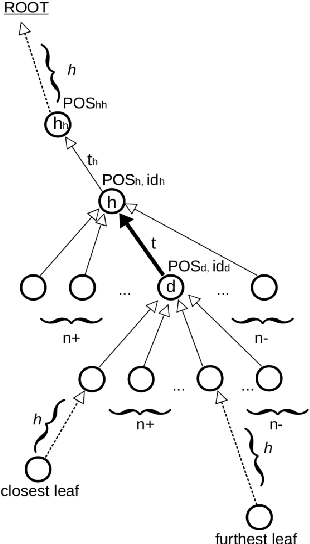
\includegraphics[scale=0.5]{img/lisca_stats.png}
    \caption[Features Used by LISCA to Calculate Plausibility Score for an Arc]{Features Used by LISCA to Calculate Plausibility Score for an Arc (marked in bold). Figure borrowed from \cite{alzetta2017dangerous}. }
\end{reusefigure}

\textbf{Add why we use CV HERE}

In the following subsections, we shall elaborate on the experiment with LISCA. We start with the specification of the dataset to be used for the experiment in section \ref{data:lisca}, followed by the elaboration on experimental setup in section \ref{preprocess:lisca}. Section \ref{arcs:focus} specifies the manner of investigation for the analysis of arcs. We report the statistics on the baseline in section \ref{baseline:lisca}, followed by analysis of cross-validation as a strategy in section \ref{compare:lisca}. Section \ref{typologies:lisca} deals with the typologies of errors discovered over the complete experiment. The chapter concludes with a discussion on the findings of the experiment in section \ref{results:lisca}.

\section{Dataset}
\label{data:lisca}

The experiment was conducted entirely on data from \verb|hi|-HDTB treebank from UDv2.4\footnote{Code alongwith manually annotated data is available at \url{https://github.com/Akshayanti/Masters-Thesis-CUNI-2020/tree/master/lisca_coldstart}} \citep{UDv2.4}. The motivation behind the limiting of the dataset to a particular language is threefold. Firstly, the treebank in question is limited to news genre. The lack of variability in the genre in the treebank can be used to frame a better statistical model than when there would be different genres present. Secondly, the treebank is medium sized (16,000+ sentences containing around 350k tokens) as can be seen in Table \ref{tab:hi_size2}. The medium sized treebank is optimal in the manner that a variety of values (of the number of folds in \(k\)-fold cross validation procedure) can be experimented with. Furthermore, the different values of the parameter can be used to ascertain the performance of the algorithm in both large-sized and small-sized treebanks. Lastly, the author has \verb|hi| as their native language, making it easier for them to analyse the given data, thus reducing the source of ambiguity during the process of manual annotation and verification of results from the results of the algorithm.

\begin{table}[h]
    \centering
    \begin{tabular}{|c|c|c|}
    \hline
    \textbf{Split} & \textbf{Sentences} & \textbf{Tokens}\\
    \hline
    \hline
    \textbf{dev} & 1 659 & 35 217\\
    \textbf{test} & 1 684 & 35 430\\
    \textbf{train} & 13 304 & 281 057\\
    \hline
    \hline
    \textbf{Total} & \textbf{16 647} & \textbf{351 704}\\
    \hline
    \end{tabular}
    \caption{Size of \texttt{hi}-HDTB treebank}
    \label{tab:hi_size2}
\end{table}

\section{Experimental Setup}
\label{preprocess:lisca}

For the remainder of the experiment, we adapt the usage of \textit{iteration} and \textit{run} as follows. The results of one \textit{run} would be analysed together. For a given \(k\) value in \(k\)-fold cross validation, the experimental data is split into \(k\) different folds, running \(k\) \textit{iterations} for one run. 

For the different runs of the current experiment, the total number of sentences poses a problem in the terms of how many folds the data can be split into\footnote{16,647 can be factorised as 3 x 31 x 179, which allows limited manipulation in the number of folds that can be worked with for equal distribution of instances.}. To combat this problem, we first concatenate the different splits of the treebank into one. The concatenated split is then downsampled to 16,000 sentences. This downsampled data becomes our functional dataset for the experiment. The downsampling is needed to allow for the different values of \(k\) to work. While the data if downsampled to 16,640 instances would have also worked, we chose to set the count to 16,000 sentences for empirical reasons. The number of sentences from the original splits that feature in the downsampled version are as listed in Table \ref{tab:split_lisca_downsample}.

\begin{table}[h]
    \centering
    \begin{tabular}{|l||c|c||c|c|}
    \hline
    \multicolumn{1}{|c||}{\textbf{Split Name}} &
    \multicolumn{2}{c||}{\textbf{Sentences}} &
    \multicolumn{2}{c|}{\textbf{Tokens}}\\
     & \textbf{Before} & \textbf{After} & \textbf{Before} & \textbf{After}\\
    \hline
    \textbf{dev} & 1 659 & 1 601 & 35 217 & 33 964\\
    \textbf{test} & 1 684 & 1 614 & 35 430 & 33 981\\
    \textbf{train} & 13 304 & 12 785 & 281 057 & 270 249\\
    \hline
    \hline
    \textbf{Total} & 16 647 & 16 000 & 351 704 & 338 194\\  
    \hline
    \end{tabular}
    \caption{Counts of Sentences and Tokens from Individual Splits, Before and After Downsampling}
    \label{tab:split_lisca_downsample}
\end{table}

\subsubsection{Setup for Baseline Run}

For establishing baseline, we train the algorithm on concatenated dev and train splits of the downsampled data, and get the plausibility scores for the data in the downsampled test split.

\subsubsection{Setup for Experimental Runs}

The experiments were conducted on 3 different values of \(k\). The chosen values were \(k = \{2, 4, 8\}\). When the values of \( k \geq 10\) were considered, the resulting data folds became smaller enough to not yield satisfactory results. Having made the choice of \(k\) values, the effective dataset was then split into folds corresponding to the \(k\) value.

For each value of \(k\), the cross-validation procedure was applied to treat each fold as test data across \(k\) different iterations. The LISCA algorithm for each iteration was run by \citeauthor{lisca} separately such that the training fold was used to train the algorithm, and then the arcs in test fold given scores as per the trained model for the iteration data. Algorithm \ref{algo:liscadata} summarises the procedure involved so far.

\begin{algorithm}[H]
\caption{Experimental Setup for \(k\)-fold Cross Validation}
\label{algo:liscadata}
    \begin{algorithmic}[1]
    \REQUIRE Downsampled \texttt{hi}-HDTB Treebank $T$
    \FORALL{$k$ in \{2, 4, 8\}}
        \STATE $T.folds \leftarrow \{T.1$, ..., $T.k\}$ subject to conditions:
        \STATE $T = \bigcup \{T.1, ..., T.k\}$ \COMMENT{Condition 1}
        \STATE $sentences(T.i) = sentences(T)/k \hspace{2mm} \forall T.i \in T$
        \COMMENT{Condition 2}
        \STATE $\bigcap \{T.x1, T.x2\} = \phi \hspace{2mm} \forall \{T.x1, T.x2\}  \in T.folds$ \COMMENT{Condition 3}
        \FOR{$iteration$ in 1, ..., k}
            \STATE $fold.test \leftarrow T.iteration$
            \STATE $fold.training \leftarrow T - T.iteration$
            \STATE $lisca.iteration \leftarrow$ trained LISCA model on $fold.training$
            \STATE Rank arcs in $fold.test$ using $lisca.iteration$
        \ENDFOR
    \ENDFOR
    \end{algorithmic}
\end{algorithm}

\section{Arcs in Focus}
\label{arcs:focus}

The evaluation of a trained LISCA model on a given test data generates several types of statistics. In addition, the individual arcs in the results of the LISCA algorithm are split into 10 equal bins in descending order of their plausibility scores, with an additional bin for the remnants. The statistics are presented on a per-bin basis and include POS distribution, deprel distribution, POS and deprel distribution, syntactic link length distribution, among others. While the per-bin statistics are a useful feature, the cross validation process in the context of current experiment does not need such per-bin statistics. Instead we focus on individual arcs and their plausibility scores in the current experiment.

Henceforth, we call a particular arc as flagged in a particular run if its plausibility score in the run is designated as 0, i.e. the arc is deemed as improbable by the run. While \cite{alzetta2017dangerous} looked at all the instances in the last two bins (and the extra remnant bin), the current setup narrows down the search scope. The last two (and the extra remnant) bins in question are the only ones containing arcs with 0-score or with scores that are very close to 0. As we would show later (in section \ref{statistics:experiments}), the scores for non-zero scored arcs would fluctuate with different datasets of the same language, or even based on the number of folds in cross validation. This can be extrapolated to state that the non-zero scored arcs in the bins in question can also vary in their scores, making the bin-specific treatment incomparable across different runs. In contrast, looking at zero-scored arcs gives us a uniform base for analysis throughout, considering that the arc was marked as improbable, and not probable with a low score.

\section{Statistics}

\subsection{Baseline Run (IN PROGRESS)}
\label{statistics:baseline}

\begin{table}[H]
    \centering
    \begin{tabular}{|l|l|}
        \hline
        \textbf{Statistic} & \textbf{Count / Value} \\
        \hline
        Total arcs & 33 739\\
        Min Score & 0.00\\
        Max Score & 1.82 E-07\\
        0-scored arcs (in \%) & 221 (0.655 \%)\\
        \hline
    \end{tabular}
    \caption{Statistics for Arc Scores in Baseline Run}
    \label{tab:stats_baseline}
\end{table}

\begin{table}[H]
    \centering
    \begin{tabular}{c|c}
         &  \\
         & 
    \end{tabular}
    \caption{Typology of Errors in Baseline Run}
    \label{tab:my_label}
\end{table}
\subsection{Experimental Runs}
\label{statistics:experiments}

Table \ref{tab:absminmax} shows the number of arcs that were flagged across different experimental runs. As mentioned earlier, the maximum score fluctuates with the different \(k\)-values across different runs, even when the overall experimental data remains the same.

\begin{table}[H]
    \centering
    \begin{tabular}{|c|c|c|c|c|}
    \hline
    \textbf{\(k\)-value} & \textbf{Min Score} & \textbf{Max Score} & \textbf{0-score arcs} & \textbf{Total arcs}\\
    \hline
    \hline
    2 & 0.00 & 1.96 E-07 & 3 487 & 336 079 \\
    4 & 0.00 & 1.93 E-07 & 2 620 & 336 079 \\
    8 & 0.00 & 1.91 E-07 & 2 319 & 336 079 \\
    \hline
    \end{tabular}
    \caption{Statistics for Arc Scores in Experimental Runs}
    \label{tab:absminmax}
\end{table}

The number of 0-scored arcs went down with an increasing \(k\)-value. In addition, all the arcs flagged in a particular run were also present in a run with a lower \(k\)-value, i.e. the arcs flagged in run with \(k=4\) were also present in \(k=2\). Similarly, the arcs flagged in run with \(k=8\) were present in the run with \(k=4\) as well as one with \(k=2\). We compare the performance of the different experimental runs against each other in section \ref{analysis:all}.

\section{Analysis (IN PROGRESS HEREAFTER)}
\label{compare:lisca}

In this section, we analyse the experiment in two parts. In the first part of the analysis (Section \ref{analysis:test}), we check the usefulness of \(k\)-fold cross validation against the arcs from only the test data. We look at the arcs that were not flagged initially by the baseline, as well as the additional arcs flagged during the different cross validation runs. The primary motive of this analysis is to understand how the cross validation technique performs in relation to the baseline task.

In the second part of the analysis (Section \ref{analysis:all}), we look at all the arcs that are flagged in different cross validation runs, regardless of them belonging to the baseline's test or train data. The motive of this analysis is to understand how the difference in number of folds during cross validation affects the flagged instances.

\subsection{Baseline vs Cross Validation: Who did it better?}
\label{analysis:test}

Table \ref{tab:test_lisca} shows the number of test arcs that were flagged across different cross validation runs. The values in column 3 represent the count of instances that were flagged by the experimental run as well as the baseline run, while the last two columns highlight the extra instances that were flagged by the experimental run, but were not flagged by the baseline run. 

\begin{table}[H]
    \centering
    \begin{tabular}{|c||c|c|c|c|}
    \hline
    \multicolumn{1}{|c||}{\textbf{\(k\)-value}} &
    \multicolumn{1}{c|}{\textbf{\# Flagged}} &
    \multicolumn{1}{c|}{\textbf{\# Also Flagged}} &
    \multicolumn{2}{c|}{\textbf{Newly Flagged}}\\
     & & \textbf{by Baseline Run} & \textbf{Error} & \textbf{No Error}\\
    \hline
    2 & 333 & 211 (63.36\%) & ? & ?\\
    4 & 254 & 205 (80.71\%) & ? & ?\\
    8 & 226 & 205 (90.71\%) & ? & ?\\
    \hline
    \end{tabular}
    \caption{Comparison of Baseline and Experimental Runs}
    \label{tab:test_lisca}
\end{table}

\begin{table}[H]
    \centering
    \begin{tabular}{|l|c|}
    \hline
    \textbf{Error Typology} & \textbf{Counts}\\
    \hline
         &  \\
         &  \\
    \hline
    \textbf{Total} & \textbf{122}\\
    \hline
    \end{tabular}
    \caption{Typology of Errors in Instances Picked by Experimental Runs, but not by Baseline}
    \label{tab:typology_experimental_not_baseline}
\end{table}


\begin{table}[H]
    \centering
    \begin{tabular}{|l|c|}
    \hline
    \textbf{Error Typology} & \textbf{Counts}\\
    \hline
         &  \\
         &  \\
    \hline
    \textbf{Total} & \textbf{10}\\
    \hline
    \end{tabular}
    \caption{Typology of Errors in Instances Picked by Baseline, but not by Experimental Runs}
    \label{tab:typology_baseline_not_experimental}
\end{table}


\subsection{Comparing Different Experimental Runs}
\label{analysis:all}

For the analysis of the different cross-validation runs, we noticed that the count of flagged instances decreased with the increase in the number of folds. We hypothesise that as we increase the number of folds, the detection of rare errors improves while the detection of frequent errors deteriorates. having noted this, we analysed the effect of each k-value in the following manner. For the 0-scored arcs that were common to all the runs, 200 randomly chosen arcs (out of 2319) were evaluated manually. Out of the arcs common only to the runs corresponding to \(k= \{2, 4\}\), 100 were randomly chosen for manual evaluation. Finally, 100 of the arcs that are local only to the run corresponding to \(k=2\) were chosen randomly for manual evaluation. The results of the manual evaluation are showcased in Table \ref{tab:liscatypology}.

\begin{table}[H]
    \centering
    \begin{tabular}{|l|c|c|c|}
        \hline
        \textbf{Error Typology} & \textbf{\(k = \{2, 4, 8\}\)} & \textbf{\(k= \{2, 4\}\)} & \textbf{\(k=2\)} \\
        \hline
        \hline
        \textbf{\texttt{acl4amod}} & 1 & 0 & 2 \\
        \textbf{\texttt{amod4xcomp}} & 5 & 2 & 2 \\
        \textbf{\texttt{auxAsHead}} & 0 & 0 & 2 \\
        \textbf{\texttt{nmod4obl}} & 3 & 0 & 5 \\
        \textbf{\texttt{obl4advcl|acl}} & 1 & 1 & 1 \\
        \texttt{advmod4amod} & 1 & 1 & 0 \\
        \texttt{nsubj4obl} & 3 & 3 & 1 \\
        \texttt{obl4xcomp} & 3 & 1 & 4 \\
        \texttt{xcomp4advmod} & 0 & 0 & 1 \\
        \texttt{Wrong Head} & 13 & 2 & 4 \\
        \texttt{Tree Error} & 23 & 1 & 3 \\
        \texttt{Random Error} & 32 & 10 & 10 \\
        No Error & 115 & 79 & 65 \\
        \hline
        \hline
        \textbf{Total Errors} & 85 (42.5 \%) & 21 (21 \%) & 35 (35 \%) \\
        \hline
    \end{tabular}
    \caption[Error Typologies for Different Folds in Experimental Runs]{Error Typologies for Different Folds in Experimental Runs. Error Typologies marked in bold have been previously pointed out by \cite{alzetta2017dangerous}.}
    \label{tab:liscatypology}
\end{table}

We estimate the normalized frequency of each error type over 1000 instances in Table \ref{tab:normalized_experimental_lisca}. The values are calculated as per Equations \ref{normalised:1} - \ref{normalised:3}. The equations estimate the normalized count based on the distribution of the errors as per manual evaluation (as reported in Table \ref{tab:liscatypology}) over the total flagged instances as per Table \ref{tab:absminmax}. The error types \texttt{Wrong Head} and \texttt{Tree Error} are propagated on the tree level, and not on the arc level\footnote{An elaborate discussion on the propagation of these errors can be made only after a discussion of the considered error type. The reader is advised to refer to Sections \ref{error:wrongHead}, \ref{error:treeError}, and the discussion in Section \ref{discussion:errorPropagation}}. Keeping this in mind, and the fact that an increase in number of folds does not increase the number of flagged instances, the normalized frequency of these errors are kept at the minimum of the calculated normalized frequency for different runs. The resulting deficit of counts is adjusted by increasing the counts of `No Error' instances.

\begin{align}
    \text{Normalized Frequency}_{error} &= C_{2} * 5 &\text{for }k=8 \label{normalised:1}\\
    & = \frac{C_{2} * 2319}{524} + \frac{C_{3} * 311}{262} & \text{for }k=4 \label{normalised:2}\\
    & = \frac{C_{2} * 23190}{6974} + \frac{C_{3} * 3110}{3487} + \frac{C_{4} * 8670}{3487}& \text{for }k=2 \label{normalised:3}
\end{align}
    where \(C_{i}\) represents the value in \(i\) -th column, corresponding to the \(error\) marked in first column in Table \ref{tab:liscatypology}.

\begin{table}[H]
    \centering
    \begin{tabular}{|l|c|c|c|}
        \hline
        \textbf{Error Typology} & \textbf{\(k = 2\)} & \textbf{\(k= 4\)} & \textbf{\(k=8\)} \\
        \hline
        \hline
        \textbf{\texttt{acl4amod}} & 8 & 4 & 5 \\
        \textbf{\texttt{amod4xcomp}} & 23 & 24 & 25 \\
        \textbf{\texttt{auxAsHead}} & 5 & 0 & 0 \\
        \textbf{\texttt{nmod4obl}} & 22 & 13 & 15 \\
        \textbf{\texttt{obl4advcl|acl}} & 6 & 6 & 5 \\
        \texttt{advmod4amod} & 4 & 6 & 5 \\
        \texttt{nsubj4obl} & 15 & 17 & 15 \\
        \texttt{obl4xcomp} & 21 & 14 & 15 \\
        \texttt{xcomp4advmod} & 2 & 0 & 0 \\
        \texttt{Wrong Head} & 55 & 55 & 55 \\
        \texttt{Tree Error} & 85 & 85 & 85 \\
        \texttt{Random Error} & 140 & 153 & 160 \\
        No Error & 614 & 625 & 615 \\
        \hline
        \hline
        \textbf{Total Errors} & 386 (38.6 \%) & 375 (37.5 \%) & 385 (38.5 \%) \\
        \hline
    \end{tabular}
    \caption[Normalized Error Frequencies for Experimental Runs]{Normalized Error Frequencies for Experimental Runs. Error Typologies marked in bold have been previously pointed out by \cite{alzetta2017dangerous}.}
    \label{tab:normalized_experimental_lisca}
\end{table}

From the table, it can be noted that an increase in the number of folds has almost no effect on the number of false positives (indicated by values corresponding to the `No Error' entry). While this could be caused by the adjustment we made for the count of the error types \texttt{Wrong Head} and \texttt{Tree Error}, 

As per Table \ref{tab:normalized_experimental_lisca}, the following errors are found to be significantly common: \texttt{amo4xcomp}, \texttt{nmod4obl}, \texttt{nsubj4obl}, \texttt{obl4xcomp}, \texttt{Wrong Head}, \texttt{Tree Error} and \texttt{Random Error}. Of these, the error types \texttt{amod4xcomp} and \texttt{nmod4obl} have been previously elaborated upon by \cite{alzetta2017dangerous}, and thus do not warrant a discussion in this document. The discussion on the error types \texttt{Wrong Head} and \texttt{Tree Error} is reserved for the final section, owing to the manner in which these errors propagate. Similarly, the discussion on \texttt{Random Error} is also limited to the final section owing to the peculiarities of the LISCA algorithm. We elaborate on the two discovered error types, viz. \texttt{nsubj4obl} and \texttt{obl4xcomp}, alongwith \texttt{Wrong Head} and \texttt{Tree Error} in the next section.

\section{Error Typologies}
\label{typologies:lisca}

In this section, we elaborate on the error typologies discovered throughout the scope of the experiment such that the discovered error type contributes to at least 1\% of the total discovered errors in any run. The focused errors in this section include: \texttt{nsubj4obl}, \texttt{obl4xcomp}, \texttt{Wrong Head}, and \texttt{Tree Error}. Since the error type \texttt{Random Error} is not systemic in nature, we do not elaborate on it.

\subsection[Confusion Between Oblique Dependent of Noun and Nominal Subject: \texttt{nsubj4obl}]{\texttt{nsubj4obl}: Confusion Between Oblique Dependent of Noun and Nominal Subject}

This error type refers to the cases where the oblique nominal dependent of a nominal subject is incorrectly marked as nominal subject. This is a relatively obscure error pattern, but nonetheless the pattern is exhibited across the data. In the example given below, \textit{Bhartiya Janta Party} is an oblique dependent of \textit{Trinamool Congress}, but has been marked wrongly as the nominal subject, as can be seen in Figure \ref{fig:lisca_nsubj4obl}. \textbf{MODIFY THIS EXAMPLE}

\begin{example}
\label{examp:lisca_hi}
\textbf{ }\\
\textbf{Text (\texttt{hi}):} \texthindi{भारतीय जनता पार्टी से दूरी बनाते हुए तृणमूल कांग्रेस ने …}\\
\textbf{Translit:} \textit{bhartiya janata party se doori banaate hue Trinamool Congress ne …}\\
\textbf{Lit.:} Bhartiya Janta Party from-\textit{Dat.} dissociating Trinamool Congress \textit{Nom.} …\\
\textbf{Translated:} Dissociating itself from Bhartiya Janta Party, Trinamool Congress …
\end{example}

\begin{figure}[h]
    \centering
    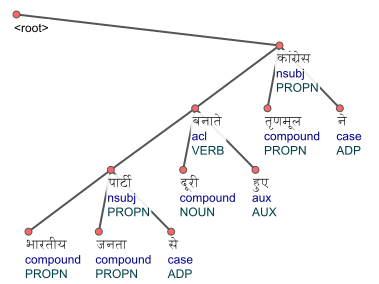
\includegraphics[scale=0.90]{img/lisca_nsubj4obl.png}
    \caption{Dependency Tree for Example \ref{examp:lisca_hi} Showing nsubj4obl Error Type.}
    \label{fig:lisca_nsubj4obl}
\end{figure}

\subsection[Confusion Between Oblique Dependent of Noun and ??: \texttt{obl4xcomp}]{\texttt{obl4xcomp}: Confusion Between Oblique Dependent of Noun and ??}


\subsection[Head Identification or Head Labelling Error: \texttt{Wrong Head}]{\texttt{Wrong Head}: Head Identification or Head Labelling Error}
\label{error:wrongHead}

While \citeauthor{alzetta2017dangerous} mention head labelling error as a sub-type of the error pattern(s), we distinguish the error type from others. In our case, we use the label to identify the cases when the associated deprel is wrong because of the selection of wrong head. The error type refers to the case where the selection of wrong head is detrimental in choice of a deprel, and where the case of deprel assignment is suspected on the basis of the relational head. This is an important distinction because there exist significant number of parsers that assign more weight to the relationships, and decide on the associated deprels accordingly.

\subsection[Multiple Annotation Errors in a Dependency Tree: \texttt{Tree Error}]{\texttt{Tree Error}: Multiple Annotation Errors in a Dependency Tree}
\label{error:treeError}

This error type can be considered as an extreme case of \texttt{Wrong Head} error. In the case of dependency trees, where multiple tokens suffer from \texttt{Wrong Head} error, it is not possible to evaluate the tree owing to disrupted tree structure. The disruptions in the tree structure can be exhibited in form of non-projectivity, multiple deprel errors, multiple head errors, among others. Essentially speaking, a tree marked with this error type requires re-annotation before any analysis can be performed on it.

\section{Results and Discussion}
\label{results:lisca}

\subsection{0-scored Arcs as Search Criteria}

In their work, \cite{alzetta2017dangerous} focused on a total of 39.7k arcs in their annotation process and were finally able to manually revised 789 arcs, giving an estimated error detection rate of 2\% from the flagged instances. In our baseline run, a focus on 221 0-scored arcs led to an estimated error detection of \textbf{?} instances \textbf{(??? \%)}. We must stress here that the results across the two experiments are NOT directly comparable since the treebanks used in the cited authors' experiment was of far superior quality than the one used in the current experiment. A lower quality treebank would imply a higher distribution of errors, and that could be the sole reason why the focus on a smaller subset gave a satisfactory error detection rate. Additionally, the size difference in the cited authors' work and the baseline task is another reason why the two approaches cannot be compared. We must also stress here that in our baseline approach, the search scope was lowered significantly (as compared to the experimental runs). To establish any significant difference between either approach, more experiments should be conducted with the same treebank (ensuring the quality of experimental data is a controlled variable) to establish the probability distribution of errors in 0-scored arcs and in the approach as utilised by \citeauthor{alzetta2017dangerous}.

\subsection{Error Propagation in case of \texttt{Tree Error} and \texttt{Wrong Head} errors}
\label{discussion:errorPropagation}

The high count of \texttt{Tree Error} can be explained by error chaining. As mentioned earlier, we designated the arcs to this error type based on the other arcs in the tree. In case a given tree contains \(x\) number of flagged arcs, there is a high possibility that all of these arcs would be flagged together under this error type, making the count swell up. Regardless, the error type can be used to flag trees in the data that are poorly annotated (since a number of arcs therein are flagged simultaneously), making the re-annotation process a lot more macro than when a single arc is flagged in a tree.

While \texttt{Tree Error} is propagated across all the arcs in the same tree, the \texttt{Wrong Head} propagates at the parent arc level. 

There is a subtle difference between error detection tools, and the inconsistency detection tools. While inconsistency detection tools do not need to find errors if they are made consistently, the error detection tools should also point at the consistent errors. Considering that LISCA bases its model on a reference, it is an inconsistency detection tool. This is the primary reason why the random errors were detected more than all the systematic errors (except that of \texttt{Wrong Head} and \texttt{Tree Error}) put together.

\subsection{Cross Validation as Strategy}

\subsection{Future Directions}

===========================================

Looking at the data obtained from Table \ref{tab:liscatypology}, we achieve \(\approx 42 \%\) precision in identification of errors when we select \(k=8\). The precision drops to \(\approx 35 \%\) when the value of \(k\) is lowered to \(k=4\). As the value of \(k\) is lowered to \(k=2\), the precision rises again to \(\approx 40 \%\). While a very high or a very low value of \(k\) can be considered optimal, we argue that the size of dataset is the determining factor in selection of value of \(k\) as discussed below:

\begin{enumerate}
    \item For the case of a very low \(k\) value, there is a slight drop in precision. This implies that the results of evaluation are likely to contain a lot of random errors, and false negatives. However, for instances where the dataset is not particularly large, a very low \(k\) value is more optimal.
    \item For the case of a very high \(k\) value, there is the problem associated with the size of the dataset. If the dataset is not big enough, the algorithm might not have been trained well enough to avail the best precision. As such, the choice of a very high \(k\) value is optimal for cases when the dataset is large enough to allow more fragmentation.
\end{enumerate}

While there were no significant error patterns that were discovered with this experiment, we tackled an essential problem that often came in the way of using LISCA. Originally, the authors of the algorithm proposed that there is another gold-standard that is needed for training LISCA, in order to correct a silver-standard. However, we show that there is no need for another gold-standard, and that the algorithm can be trained on the silver-standard data itself in case of a missing gold-standard. This is essential since for low-resource languages where the errors need to be mined, and corrected; there is more often than not, a lack of gold-standard data. The algorithm can still be used for such cases, by selecting a low/high value of \(k\) for \(k\)-fold cross validation procedure.